\documentclass[../report.tex]{subfiles}
\begin{document}
\section{Test the model}
Upon the completion of the validation and final training phases, we proceed to the model assessment stage. In this phase, we conduct a comprehensive evaluation of the model using data samples that the model has not encountered during training. This assessment is crucial for determining the model's generalization capabilities.
\subsection{Testing Methodologies}
It is considered good practice to utilize the same metrics during testing as those employed during validation. The testing method is a function of the \href{https://github.com/cMancio00/Super-Resolution/blob/main/SRM/network.py}{\textbf{SuperResolution}} class. As illustrated in Listing \ref{lst:test}, we set the model to evaluation mode (which prevents weight updates) and compute the L1 loss and Peak Signal-to-Noise Ratio (PSNR) on the test dataset.\\
Validation and testing essentially execute the same code; however, their purposes are distinct.

\begin{lstlisting}[style=python, language=python, label={lst:test}, caption={Testing Method}]
def test(self, loss_fn, test_dataloader, device='cpu'):
	self.to(device)
	self.eval()
	total_loss = 0.0
	total_psnr = 0.0
	for low_res, high_res in test_dataloader:
	low_res = low_res.to(device)
	high_res = high_res.to(device)
	with torch.no_grad():
	predicted_high_res = self(low_res)
	loss = loss_fn(predicted_high_res, high_res)
	total_loss += loss.item()
	total_psnr += peak_signal_noise_ratio(predicted_high_res, high_res)
	
	avg_loss = total_loss / len(test_dataloader)
	avg_psnr = total_psnr / len(test_dataloader)
return avg_loss, avg_psnr
\end{lstlisting}
A comparison of the results obtained from testing and validation is presented in Table \ref{tab:test_results}, with the validation results included solely for reference. Additionally, Figure \ref{fig:test} provides a visual comparison of the test results.
\begin{table}[H]
	\centering
	\caption{Comparison of Test and Validation Metrics}
	\begin{tabular}{@{}lcc@{}}
		\toprule
		\textbf{Metric} & \textbf{Validation} & \textbf{Testing} \\ \midrule
		L1 Loss         & 0.017452            & 0.012140         \\ 
		PSNR            & 30.2676 dB         & 32.9143 dB       \\ 
		\bottomrule
	\end{tabular}
	\label{tab:test_results}
\end{table}
\begin{figure}[H]
	\caption{Test output for large model}
	\centering
	\label{fig:test}
	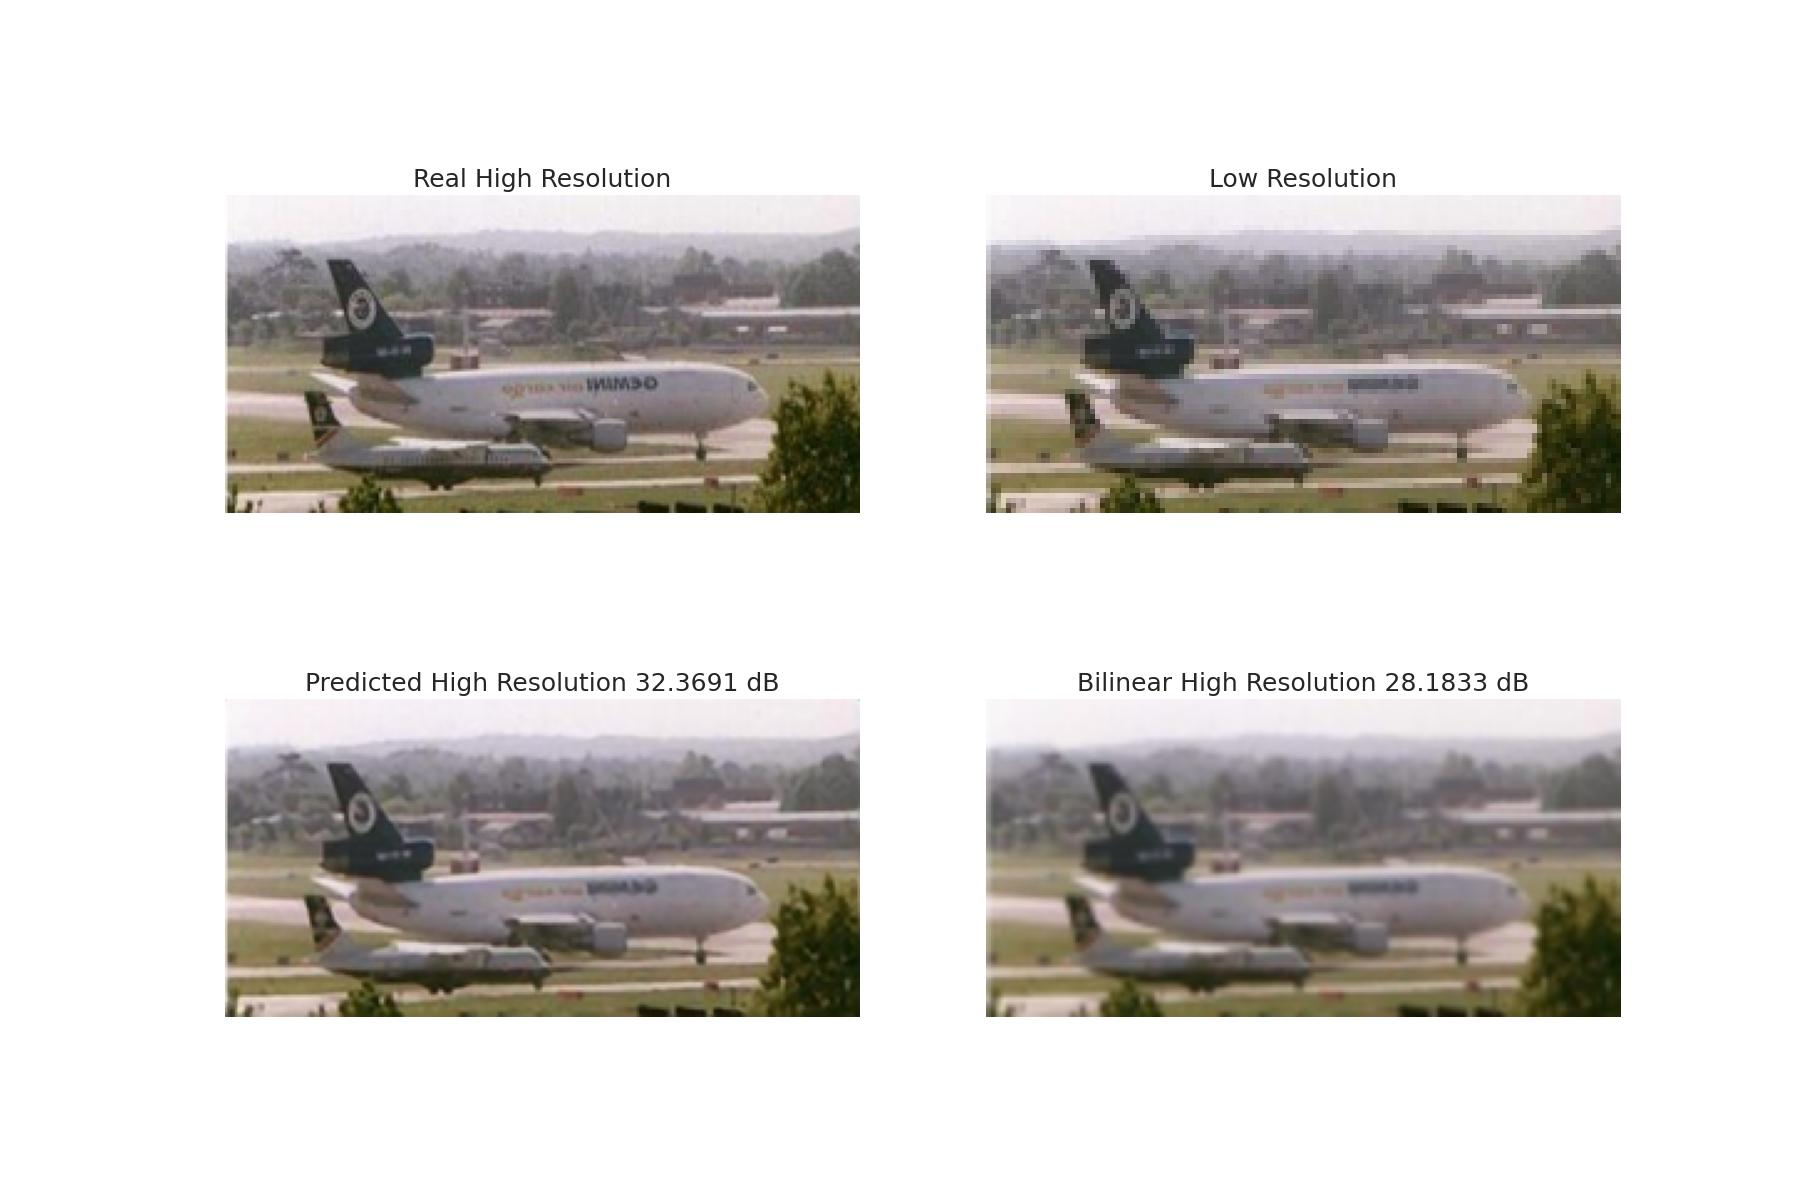
\includegraphics[width=\textwidth]{../images/test_prediction_comparison_large_model.jpg}
\end{figure}

\begin{figure}[H]
	\caption{Test output for small model}
	\centering
	\label{fig:test_small}
	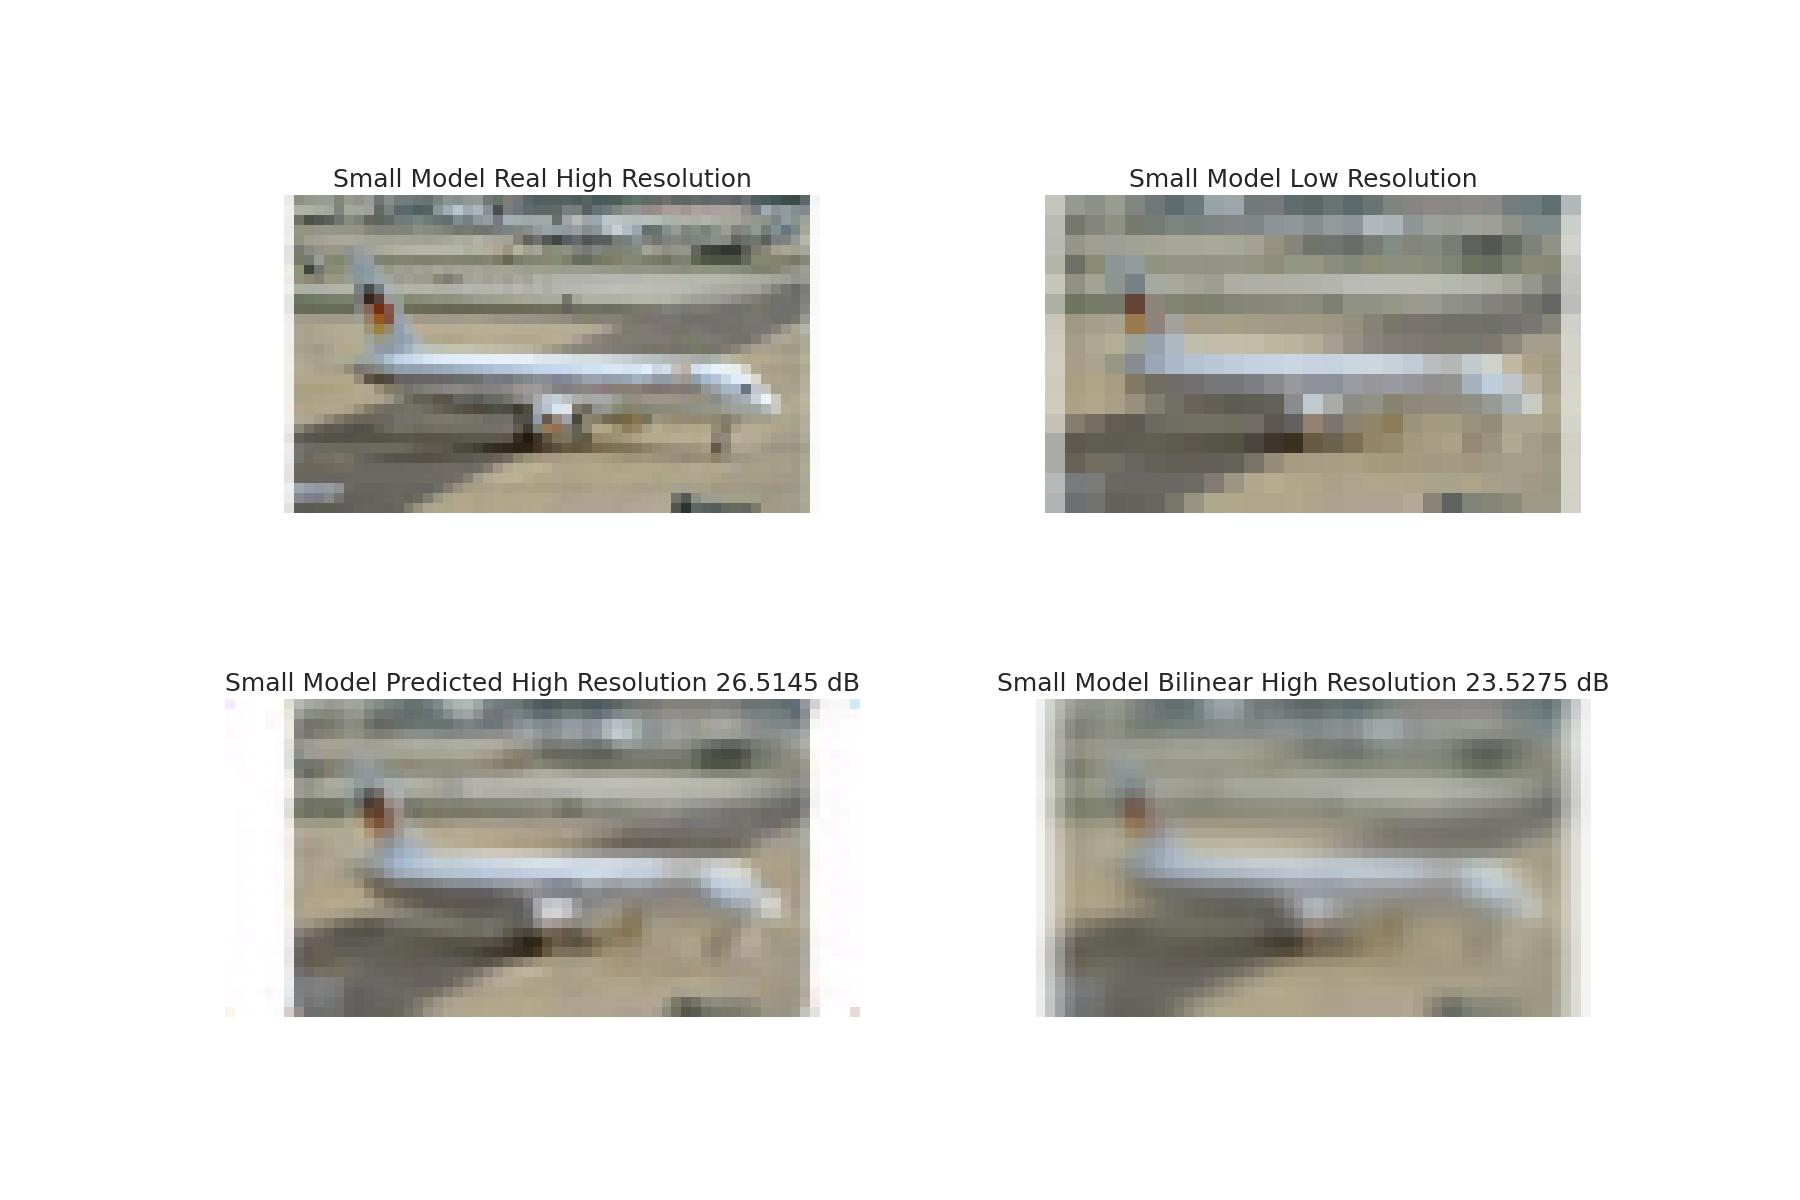
\includegraphics[width=\textwidth]{../images/test_prediction_comparison_small_model.jpg}
\end{figure}
We focused on images of airplanes seen from the front. Even though these images had low resolution, we were able to achieve good upscaling results in a relatively short time, about 12 seconds per epoch on a 3050 Ti GPU. This shows that the model works well for improving image quality while being efficient.
For the small model, we can also achieve inference in about 20 seconds on CPU, and the results are very satisfying, as the upscaling is more noticeable due to the very low resolution of the images.
\end{document}